% Chapter 6
\chapter{Motion-Robust and Ambient Light-Immune Remote PPG} % Main chapter title

\label{Chapter6} % For referencing the chapter elsewhere, use \ref{Chapter1}

\lhead{Chapter 6. \emph{Fundamental Mathematics}} % This is for the header on each page - perhaps a shortened title

%----------------------------------------------------------------------------------------
\section {Photoplethysmogram PPG \cite{wiki-PPG}}
\begin{figure}[hb]
  \centering
    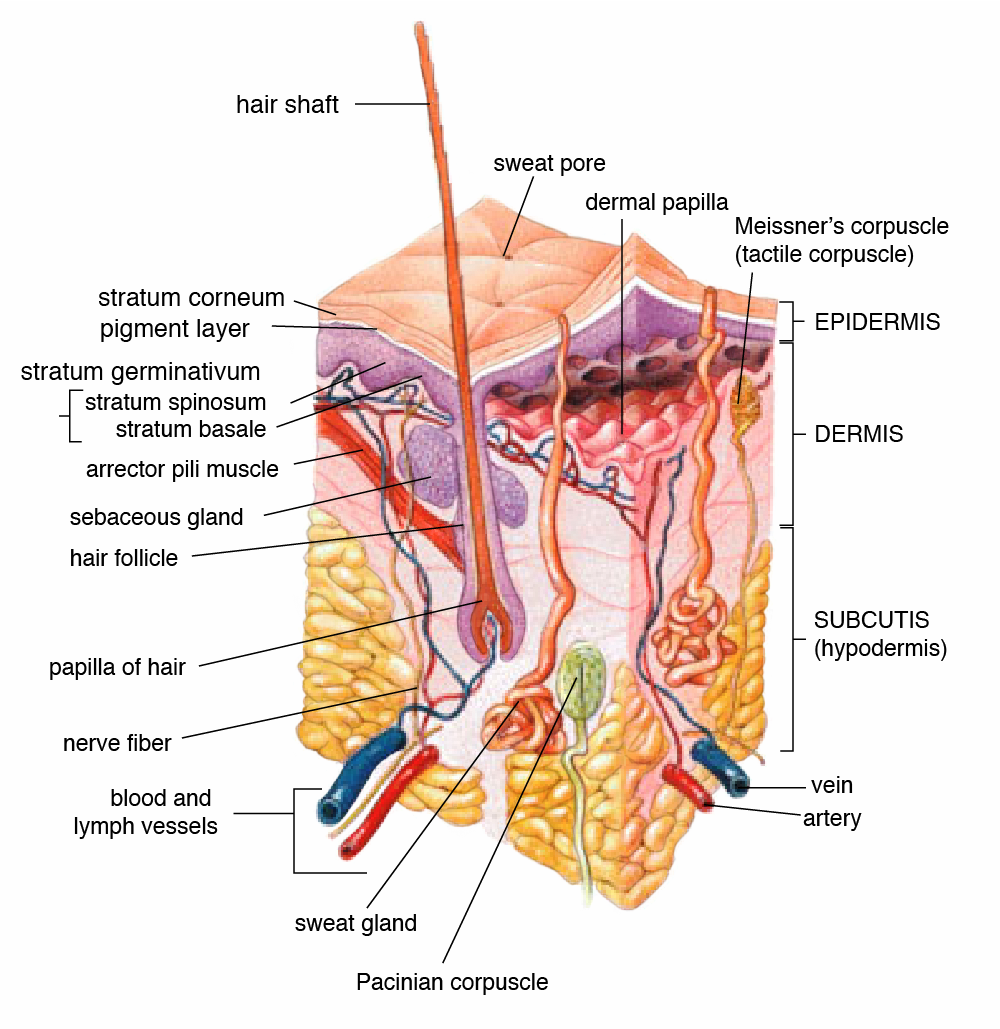
\includegraphics[width=0.7\textwidth, keepaspectratio=true]{chap6-Skinppg.png}
  \caption{Diagram of the layers of human skin.}
  \label{fig:chap6-Skinppg}
\end{figure}

A photoplethysmogram (PPG) is an optically obtained plethysmogram, a volumetric measurement of an organ.
A PPG is often obtained by using a pulse oximeter which illuminates the skin and measures changes in light absorption.
A conventional pulse oximeter monitors the perfusion of blood to the dermis and subcutaneous tissue of the skin.

Diagram of the layers of human skin \autoref{fig:chap6-Skinppg} With each cardiac cycle the heart pumps
blood to the periphery. Even though this pressure pulse is somewhat damped
by the time it reaches the skin, it is enough to distend the arteries and
arterioles in the subcutaneous tissue.

The change in volume caused by the pressure pulse is detected by illuminating the skin
with the light from a light-emitting diode (LED) and then measuring the amount of
light either transmitted or reflected to a photodiode.
Each cardiac cycle appears as a peak, as seen in the \autoref{fig:chap6-PVC}.
Because blood flow to the skin can be modulated by multiple other physiological systems,
the PPG can also be used to monitor breathing, hypovolemia,
and other circulatory conditions.

Sites for measuring PPG
While pulse oximeters are a commonly used medical device the PPG derived from them is
rarely displayed, and is nominally only processed to determine heart rate.
PPGs can be obtained from transmissive absorption (as at the finger tip) or
reflection (as on the forehead).

Motion artifacts have been shown to be a limiting factor preventing accurate readings
during exercise and free living conditions.
\begin{figure}[h]
  \centering
    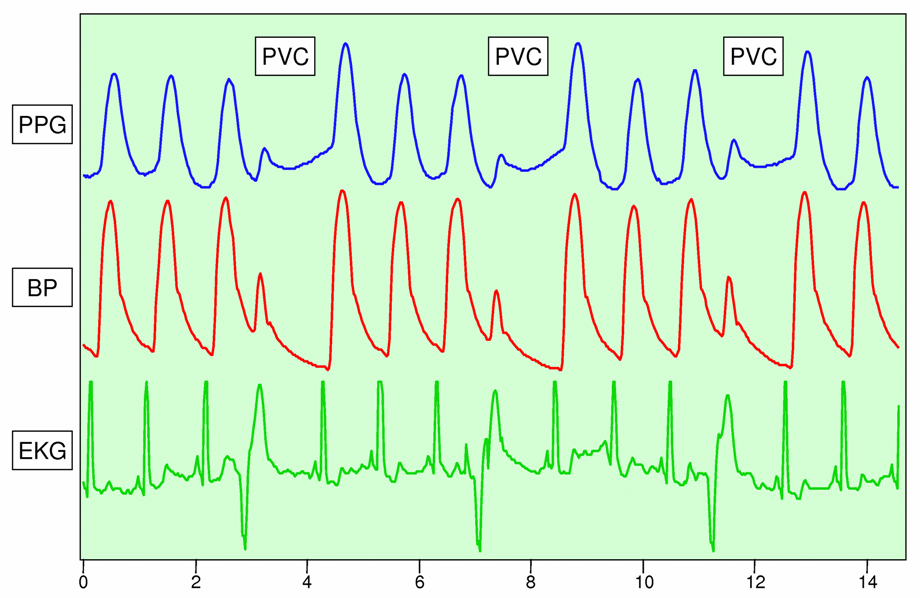
\includegraphics[width=0.7\textwidth, keepaspectratio=true]{chap6-PVC.png}
  \caption{Diagram of the layers of human skin.}
  \label{fig:chap6-PVC}
\end{figure}

%----------------------------------------------------------------------------------------
\section{The future study}

\begin{compactitem}
\item {Highly Dynamic Ambient Light Scenario}\cite {6799899}\\
Heart rate can be monitored remotely using regular RGB cameras by analyzing minute skin color changes caused
by periodic blood flow. I will study an infrared-based alternative for light-robust camera-based heart
rate measurements. It is possible to remotely measure heart rate using regular RGB cameras.
Heart rate is captured using remote photoplethysmography (remote PPG), which is an extension of the contact
photoplethysmography developed in the 1930s by Hertzman. The principle behind this
technology is that the light reflected from the skin is modulated according to the specific absorption
spectrum of the hemoglobin, the main constituent of blood. Each time the heart beats,
a new blood flow reaches the skin leading to minute variations of the skin color, so called micro-blushes.
While these micro-blushes cannot be observed by the human eye, regular camera and dedicated algorithms
allow their extraction. Results reported on remote PPG-based heart rate measurement have so far shown good
accuracy under stable light conditions for situations ranging from monitoring stationary subjects.
However, since remote PPG is based on the analysis of minute color changes, its performance in an
highly dynamic ambient light or dark setting using an RGB implementation is questionable.
The reason for concern is the highly dynamic and unpredictable environment especially in terms of lighting
conditions which can vary from (i) full to cloudy sunlight, (ii) natural to artificial light and (iii)
presence to absence of light. The amount and spectral content of the light available in the environment
are the main factors that need to be accounted for to achieve light robust camerabased heart rate measurements.
We will study an infrared-based implementation of remote PPG measurement suitable for the highly dynamic ambient light
environment and present results obtained under highly dynamic light
conditions.

\item {INFRARED-BASED REMOTE PPG}\\
As in full darkness RGB cameras do not function at all, we will study
an infrared-based remote PPG solution that uses a dedicated light source.
A light source emitting in the infrared region of the spectrum
(700nm to 1000nm) (i) ensures user comfort, as it is invisible to human
eye, and (ii) allows remote PPG measurements as the infrared region is
also modulated by the blood pulse.  Disturbances in the measurement caused
by external light sources are largely eliminated by using a narrowband
optical filter. The infrared light source is flashed in sync with the
camera frame rate. The flash duration and intensity are optimized such
that the total projected optical power complies with official safety
regulations. The extraction of the remote PPG waveform is performed by applying
spatio-temporal,  FFT, processing techniques.
To ensure that the processing takes into account only relevant pixels a
skin detection step is added. The extraction of the heart rate values from
the raw waveform is based on Fourier analysis.\cite{rPPG7005489}

\item{Future Study to combine both motion-robust and Ambient Light Immunity}

\begin{figure}[h]
  \centering
    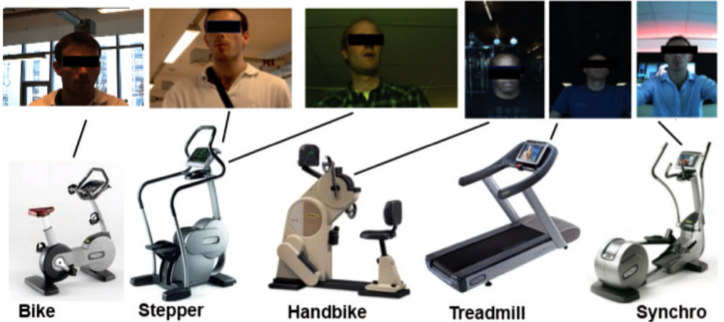
\includegraphics[width=0.7\textwidth, keepaspectratio=true]{chap6-rPPGMotion.png}
  \caption{Fitness devices and corresponding camera view to test motion robustness.}
  \label{fig:chap6-rPPGMotion}
\end{figure} \cite{rPPGPubMed}

\end{compactitem}
%----------------------------------------------------------------------------------------